\section{Kết quả thực nghiệm}

\subsection{Kết quả nội suy từng chỉ số (LOO-CV $R^2$)}
\label{sec:r2}
Sáu chỉ số nội suy được kiểm định chéo Leave-One-Station-Out trên cả hai vùng và hai bộ feature. Hình~\ref{fig:r2all} trực quan toàn bộ; phân hạng theo chính sách 3 mức bên dưới.

\begin{figure}[h]
\centering
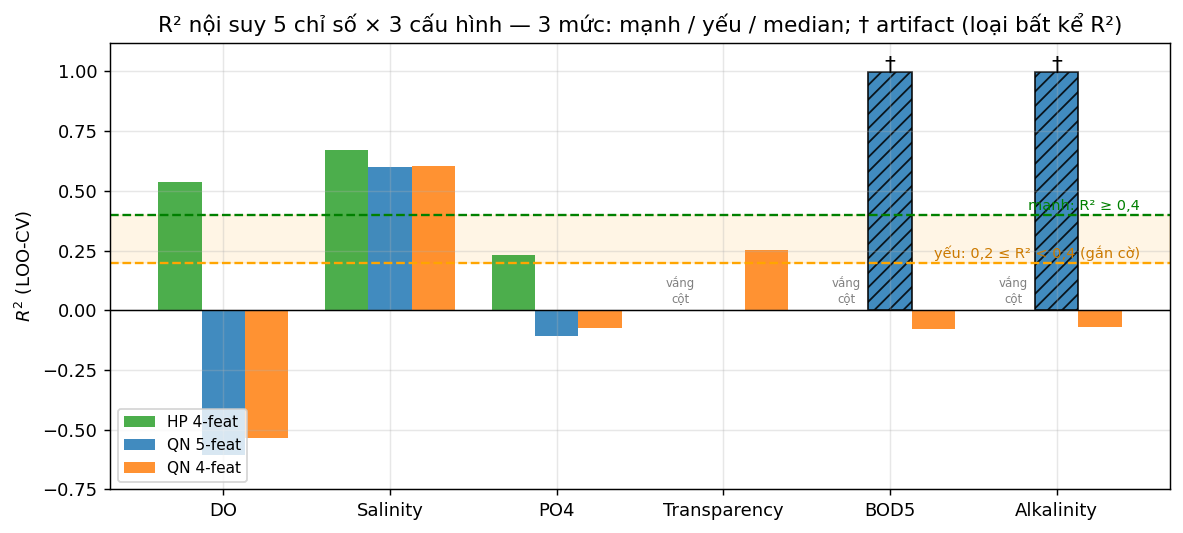
\includegraphics[width=\linewidth]{../figures/r2_all.png}
\caption{$R^2$ của 6 chỉ số $\times$ 3 cấu hình. \textbf{DO (HP)} và \textbf{Salinity (cả 2 vùng)} vượt ngưỡng $0{,}4$ một cách \emph{thực}. Hai cột gạch chéo ($\dagger$ BOD5/Alkalinity ở QN 5-feat) chạm $\approx1{,}0$ nhưng là artifact (Mục~\ref{sec:thaoluan}). Cột ``vắng cột'' = chỉ số đó không có trong dữ liệu HP.}
\label{fig:r2all}
\end{figure}

\textbf{Chính sách 3 mức tin cậy.} Thay vì một ngưỡng cứng, chỉ số được phân hạng theo $R^2$:
\begin{itemize}[nosep]
  \item \textbf{ML-mạnh} ($R^2\ge0{,}4$): dùng model, tin.
  \item \textbf{ML-yếu} ($0{,}2\le R^2<0{,}4$): dùng model \emph{nhưng gắn cờ ``độ tin thấp''} ở xuất xứ.
  \item \textbf{Median} ($R^2<0{,}2$): trung vị vùng.
  \item \textbf{Artifact} (BOD5, Alkalinity): loại \emph{bất kể} $R^2$ (xem dưới).
\end{itemize}

\begin{table}[h]
\centering\small
\caption{$R^2$ kiểm định chéo + hạng tin cậy mỗi chỉ số. HP 5-feat = 4-feat (HP không có cột COD).}
\label{tab:r2}
\begin{tabular}{lcccl}
\toprule
\textbf{Chỉ số} & \textbf{HP (4-feat)} & \textbf{QN 5-feat} & \textbf{QN 4-feat} & \textbf{Hạng / kết quả dùng} \\
\midrule
DO            & \textbf{0{,}535} & $-0{,}606$ & $-0{,}537$ & HP: \textbf{ML-mạnh}; QN: median \\
Salinity      & \textbf{0{,}673} & \textbf{0{,}599} & \textbf{0{,}602} & \textbf{ML-mạnh cả 2 vùng} \\
PO4           & $0{,}233$ & $-0{,}108$ & $-0{,}074$ & HP: \textbf{ML-yếu} (cờ); QN: median \\
Transparency  & --- & $-0{,}003$ & $0{,}254$ & QN: \textbf{ML-yếu} (cờ); HP: vắng cột \\
BOD5          & --- & $0{,}9999^\dagger$ & $-0{,}078$ & \textbf{artifact} $\to$ median \\
Alkalinity    & --- & $0{,}9995^\dagger$ & $-0{,}072$ & \textbf{artifact} $\to$ median \\
\bottomrule
\end{tabular}

{\footnotesize ``---'' = data HP không có cột. $^\dagger$ artifact COD-driven, loại bất kể $R^2$ (Mục~\ref{sec:thaoluan}).}
\end{table}

\textbf{Đọc theo từng chỉ số:}
\begin{itemize}[nosep]
  \item \textbf{DO} --- chỉ số quan trọng nhất. HP-only $R^2=0{,}535$ (ML-mạnh); QN $<0$ (median).
  \item \textbf{Salinity} --- chỉ số quan trọng \emph{thứ hai} (importance\_rank 4), \textbf{đoán được mạnh ở CẢ hai vùng} ($0{,}673$ HP, $0{,}60$ QN). Hợp lý vật lý: gradient cửa sông (nước ngọt vào $\to$ độ muối $\downarrow$, dinh dưỡng/đục $\uparrow$). Ban đầu để median do giả định sai; data đính chính.
  \item \textbf{PO4} --- HP $0{,}233$ rơi vào \textbf{ML-yếu}: dùng nhưng gắn cờ độ tin thấp (chỉ tốt hơn median $\sim$12\% RMSE). QN âm.
  \item \textbf{Transparency} --- HP không có cột; QN 4-feat $0{,}254$ là \textbf{ML-yếu} (dùng cho trạm QN, có cờ).
  \item \textbf{BOD5, Alkalinity} --- QN 5-feat $\approx1{,}0$ nhưng \textbf{artifact}: tương quan tất định với COD (Mục~\ref{sec:thaoluan}); bỏ COD thì $R^2$ rớt âm. \emph{Loại bất kể} $R^2$ cao.
\end{itemize}

\warnbox{\textbf{Tổng kết nội suy (chính sách 3 mức):} \textbf{2 mạnh} (DO ở HP, Salinity ở cả 2 vùng) $+$ \textbf{2 yếu có cờ} (PO4 ở HP, Transparency ở QN); BOD5/Alkalinity loại do artifact. Riêng trạm \textbf{Cát Bà} (HP, 4-feat): DO (mạnh) $+$ Salinity (mạnh) $+$ PO4 (yếu) $= 3$ chỉ số ML-grounded, phần còn lại median. Đặc biệt Salinity --- chỉ số quan trọng thứ 2 --- chuyển từ hằng số sang model-grounded, vá một phần hạn chế H2.}

\textbf{Phát hiện then chốt (Luồng 2):} tách \textbf{HP-only} \emph{cứu} được DO từ $R^2<0$ (gộp QN+HP) lên $R^2=0{,}535$ (Hình~\ref{fig:do}). \textbf{Luồng 1:} DO ở HP đoán được \emph{ngang nhau} ở cả 5-feature lẫn 4-feature (cùng $0{,}535$, vì HP vốn không có cột COD), nên trạm Cát Bà vẫn có DO \emph{model-grounded} kể cả khi COD chết --- đúng ô \textbf{HP-only $\times$ 4-feat} (Bảng~\ref{tab:hailuong}).

\begin{figure}[h]
\centering
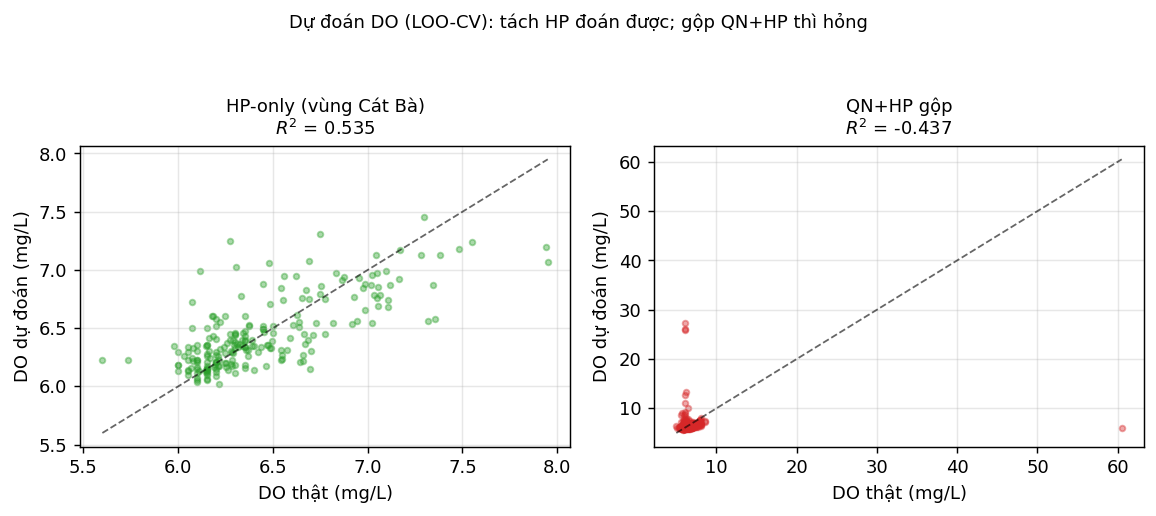
\includegraphics[width=\linewidth]{../figures/do_per_region.png}
\caption{Dự đoán DO (LOO-CV). HP-only: điểm bám đường chéo, $R^2=0{,}535$. Gộp QN+HP: phân tán, $R^2<0$ (tệ hơn trung vị). Tách vùng là yếu tố quyết định.}
\label{fig:do}
\end{figure}

\subsection{Vì sao các chỉ số còn lại để median --- bằng chứng}
\label{sec:median-evidence}
Quyết định để các chỉ số còn lại (kim loại nặng, Coliform, H2S, COD) dùng trung vị \emph{không} phải võ đoán --- chúng tôi đã chạy LOO-CV cho \emph{tất cả} (Hình~\ref{fig:medr2}). Kết quả:
\begin{itemize}[nosep]
  \item \textbf{Salinity là ngoại lệ duy nhất} đoán được ổn định cả 2 vùng ($R^2\approx0{,}6$) $\Rightarrow$ đã chuyển sang ML-target.
  \item \textbf{Kim loại QN} (As, Cd, Pb, Cu, Hg, Zn, Cr): $R^2$ đều $<0{,}2$ (phần lớn âm) --- không có tín hiệu từ 4 input sensor (kim loại đến từ nguồn thải, không liên quan pH/nhiệt/NH3/TSS).
  \item \textbf{Vài kim loại HP} ($R^2>0{,}2$: Cu, Zn, As) là \emph{nhiễu}: cột gần-LOD (median $\approx0$, phương sai bé) và \textbf{không lặp lại} ở QN (97 trạm) --- không đáng tin.
  \item \textbf{Cd, Pb, Total\_Cr ở HP}: $R^2=1{,}0$ \emph{degenerate} --- cột hằng số (phương sai 0); median đã bằng đúng hằng số đó nên ML vô nghĩa.
  \item \textbf{Coliform, H2S, COD}: $R^2<0$.
\end{itemize}

\begin{figure}[h]
\centering
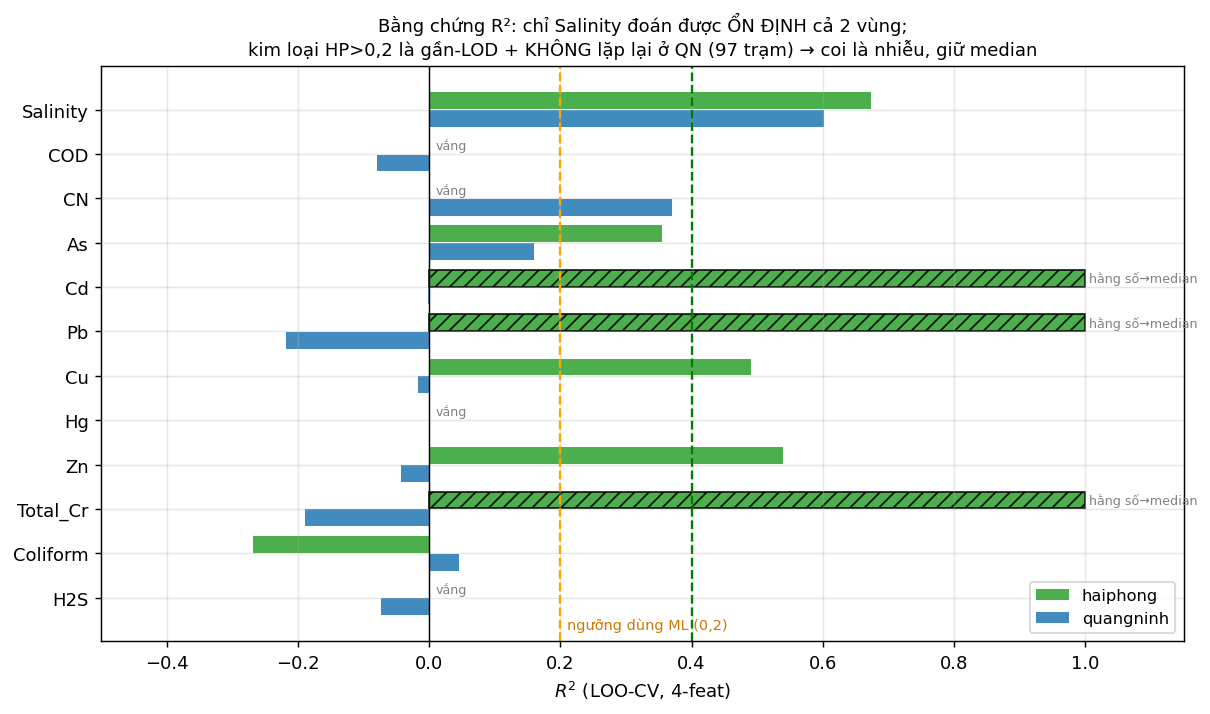
\includegraphics[width=\linewidth]{../figures/median_params_r2.png}
\caption{LOO-CV $R^2$ của các chỉ số median-default. Chỉ Salinity vượt ngưỡng ở cả 2 vùng. Kim loại HP có $R^2>0$ nhưng gần-LOD và không lặp lại ở QN; ba cột gạch chéo là hằng số ($R^2=1{,}0$ degenerate).}
\label{fig:medr2}
\end{figure}

\subsection{Chạy CLI thực tế}
Bộ test: \textbf{37/37 PASS}. Hai ví dụ báo cáo (trạm Cát Bà, vùng HP):

\begin{lstlisting}
# Ngay 2026-06-20 (COD chet -> 4feat, vung haiphong)
COD sensor: INVALID
[MONITORING] NH3 0.0068 (QCVN <=0.1) OK | pH 7.89 (6.5-8.5) OK
             Temp 30.2 EXCEED | TSS 75.8 EXCEED
[CLASSIFICATION - COBIA | vung haiphong] Score 0.900 -> "Phu hop"
  feature_set: 4feat | imputed_fraction: 71%
  ML-manh (R2>=0.4): DO, Salinity | ML-yeu (0.2<=R2<0.4): PO4
  imputed = {DO: 6.20 (manh), Salinity: 30.34 (manh), PO4: 0.042 (yeu)}
  defaulted = {As, Cd, Pb, Cu, ...}   # kim loai/Coliform/H2S -> median

# Ngay 2026-06-01 (COD song -> 5feat)
COD sensor: VALID
[MONITORING] COD 9.8 (QCVN <=10) OK | ...
[CLASSIFICATION - COBIA] Score 0.953 -> "Rat phu hop" | feature_set: 5feat
\end{lstlisting}

Phần giám sát QCVN hoạt động đúng: ngày 20/06 báo Temp và TSS vượt ngưỡng, COD bị QC loại nên không báo EXCEED giả. Phần phân loại tuy chạy nhưng cần đọc kèm các hạn chế ở mục sau.
